% !TEX root = ../../I4PRJ, Grp3 - Dokumentation.tex
I dette afsnit beskrives designet af softwarepakken Smartpool.Application.Presentation. Denne pakke indeholder præsentationslogikken, som indgår i applikationslager i det distribuerede system.

I præsentationslaget designes en række presenter-interfaces. Disse presenters har til formål at binde model- og view-lag sammen, samt at definere den tilhørende præsentationslogik. Konkrete presenter-klasser er også designet i dette lag. De konkrete klasser implementerer de førnævnte interfaces, samt benytter sig af modellen beskrevet i forrige afsnit. Der defineres også en række view-interfaces. Disse interfaces benyttes og implementeres af view klasser i de platform-specifikke udgaver af Smartpool applikationen. Interfaces er designet undervejs i projektudviklingsforløbet, i takt med at user stories er blevet åbnet og løst.

\subsubsection{Presenter-interfaces}
Presenter-interfacene definerer en simpel protokol mellem view og presenter. De indeholder metoder som bør kaldes af det tilhørende view, når bestemte events sker i view-laget. Overordnede presenter interfaces er i løbet af projektforløbet blevet identificeret, og segregeret fra de øvrige interfaces.

\begin{figure}
	\centering
	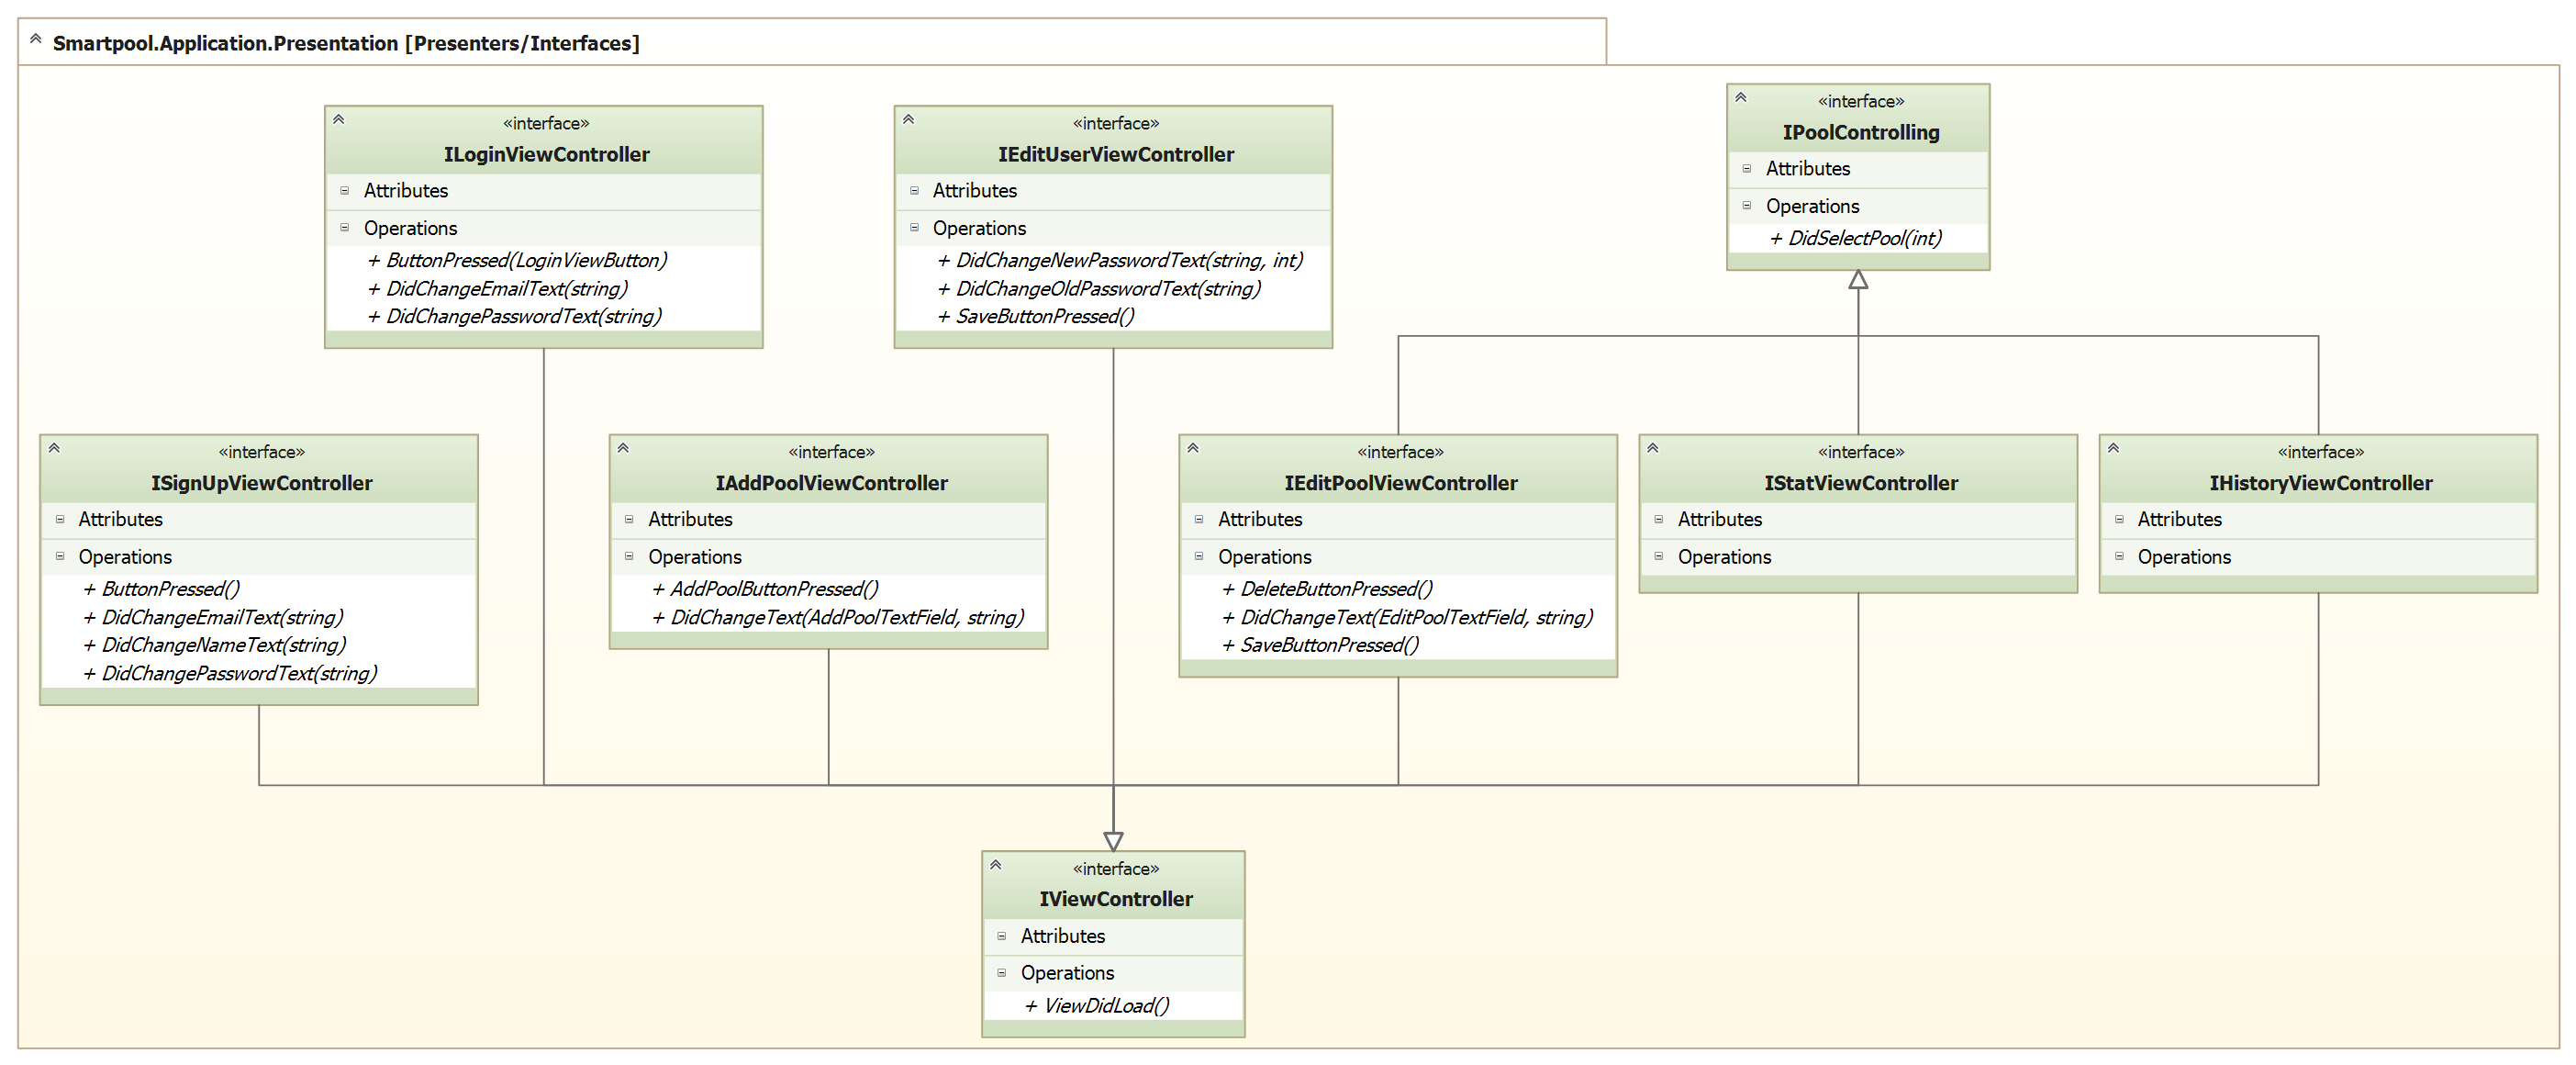
\includegraphics[width=1.0\linewidth]{figs/design/application_presentation_interfaces}
	\caption{Presenter interfaces}
	\label{fig:application_presentation_interfaces}
\end{figure}

I de efterfølgende afsnit beskrives designet af de forskellige presenter-interfaces.

\paragraph{IViewController}
IViewController interfacet er det mest generelle presenter-interface, som implementeres af alle de andre presenter-interfaces. Interfacet indeholder en metode, ViewDidLoad, som kaldes af det tilhørende view, efter view´et er loaded i hukommelsen og vises for brugeren.

\begin{figure}
	\centering
	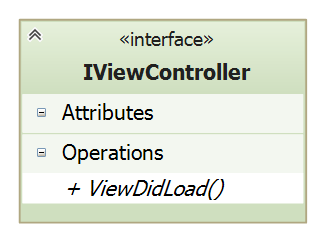
\includegraphics[width=0.3\linewidth]{figs/design/application_iviewcontroller}
	\caption{IViewController}
	\label{fig:application_iviewcontroller}
\end{figure}

\paragraph{IPoolControlling}
IPoolControlling er et interface der er segregeret fra de interfaces som håndterer visning og styring af pool oplysninger. Interfacet indeholder en metode, DidSelectPool(int), som bør kaldes af det tilhørende view, efter en pool er valgt i view´et, fra en liste eller lignende. Integer parameteren repræsenterer indekset på den valgte pool, i listen af pools (se Session).  
\begin{figure}
	\centering
	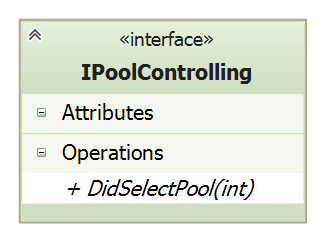
\includegraphics[width=0.3\linewidth]{figs/design/application_ipoolcontrolling}
	\caption{IPoolControlling}
	\label{fig:application_ipoolcontrolling}
\end{figure}

\paragraph{ISignUpViewController}
Interfacet er designet i forbindelse med user stories, der omhandler, at brugeren skal kunne oprette sig i systemet. Interfacet indeholder metoder, som det tilhørende view kan kalde, når events som tekst-input sker. Dermed kan presenteren, der implementerer interfacet få opdateringer fra viewet, når brugeren indtaster sine oplysninger.

\begin{table}
	\centering
	\begin{tabular}{| l | p{0.65\linewidth} |}
		\toprule
		\textbf{Klassemedlem}	& \textbf{Beskrivelse} \\
		\midrule
		+ ButtonPressed()				& En metode der kaldes af presenterens view, når brugeren fra view'et vælger at færdiggøre brugeroprettelsen.	\\\hline
		+ DidChangeEmailText(...) 			& Metoder der skal kaldes af view?et, når brugeren har indtastet tekst i de pågældende tekstfelter. \\
		+ DidChangeNameText(...)  			& \\\hline
		+ DidChangePasswordText(...) 				& En metode der kaldes af presenterens view, når brugeren indtaster sit ønskede password fra view'et. Passwordet skal indtastes to gange i view?et for at sikre, at det er korrekt indtastet. Metoden indeholder derfor en integer parameter som sættes til enten 0 eller 1, efter hvilken gang passwordet er indtastet. \\
		\bottomrule
		\end{tabular}
	\caption{Beskrivelse af ISignUpViewController-klassens medlemmer}
	\label{tab:table_design_isignupviewcontroller}	
\end{table}

\paragraph{ILoginViewController}
ILoginViewController interfacet implementeres af den presenter, der håndterer brugerens loginanmodninger. Interfacet indeholder metoder, som view?et kan kalde, når events som tekst-input sker.

\begin{table}
	\centering
	\begin{tabular}{| l | p{0.65\linewidth} |}
		\toprule
		\textbf{Klassemedlem}	& \textbf{Beskrivelse} \\
		\midrule
		+ ButtonPressed()				& En metode der kaldes af presenterens view, når en brugeren trykker på en knap eller et link i view?et. Metoden indeholder en parameter, som er en enumeration over de knapper der kan eksistere i et login view.	\\\hline
		+ DidChangeEmailText(...) 			& Metoder der skal kaldes af view?et, når brugeren har indtastet tekst i de pågældende tekstfelter. \\
		+ DidChangePasswordText(...) 				& \\
		\bottomrule
		\end{tabular}
	\caption{Beskrivelse af ILoginViewController-klassens medlemmer}
	\label{tab:table_design_iloginviewcontroller}	
\end{table}

\paragraph{IAddPoolViewController}
Dette interface er designet i forbindelse med user stories, der omhandler oprettelse af pools, på en brugers konto. Interfacet indeholder metoder, som view?et kan kalde, når events som tekst-input sker.

\begin{table}
	\centering
	\begin{tabular}{| l | p{0.65\linewidth} |}
		\toprule
		\textbf{Klassemedlem}	& \textbf{Beskrivelse} \\
		\midrule
		+ AddPoolButtonPressed()				& En metode der kaldes af presenterens view, når brugeren ønsker at gennemføre oprettelsen af poolen.	\\\hline
		+ DidChangeText(...) 					& En metode der kaldes af view?et, når brugeren indtaster tekst i et af view?ets tekstfelter. Teksten sendes  sammen med tekstfeltets id. \\
		\bottomrule
		\end{tabular}
	\caption{Beskrivelse af IAddPoolViewController-klassens medlemmer}
	\label{tab:table_design_iaddpoolviewcontroller}	
\end{table}

\paragraph{IEditUserViewController}
Dette interface er designet i forbindelse med user stories, der omhandler redigering af brugeroplysninger. Interfacet er i første omgang designet ud fra en enkelt user story, der omhandler ændring af brugens password. Interfacet indeholder der metoder, som view?et kan kalde, når brugeren indtaster ønskede password ændringer.

\begin{table}
	\centering
	\begin{tabular}{| l | p{0.6\linewidth} |}
		\toprule
		\textbf{Klassemedlem}	& \textbf{Beskrivelse} \\
		\midrule
		+ DidChangeNewPasswordText(...)				& En metode der kaldes af view?et, når brugeren indtaster sit nye password. Passwordet skal indtastes to gange i view?et for at sikre, at det er korrekt indtastet. Metoden indeholder derfor en integer parameter som sættes til enten 0 eller 1, efter hvilken gang passwordet er indtastet.	\\\hline
		+ DidChangeOldPasswordText(...)				& En metoder der skal kaldes af view?et, når brugeren indtaster sit gamle password. \\\hline
		+ SaveButtonPressed() 					& En metode der kaldes af view?et, når brugeren ønsker at gennemføre sin oprettelse. \\
		\bottomrule
		\end{tabular}
	\caption{Beskrivelse af IEditUserViewController-klassens medlemmer}
	\label{tab:table_design_iedituserviewcontroller}	
\end{table}

\paragraph{IEditPoolViewController}
IEditPoolViewController interfacet er designet i forbindelse med user stories der omhandler redigering af pools, på en brugers konto.

\begin{table}
	\centering
	\begin{tabular}{| l | p{0.7\linewidth} |}
		\toprule
		\textbf{Klassemedlem}	& \textbf{Beskrivelse} \\
		\midrule
		+ DeleteButtonPressed()				& Metoder der kaldes når brugeren vælger at slette eller gemme ændringer for en given pool.	\\
		+ SaveButtonPressed				& \\\hline
		+ DidChangeText(...) 					& En metode der kaldes af view?et, når brugeren indtaster tekst i et af view?ets tekstfelter. Teksten sendes  sammen med tekstfeltets id. \\
		\bottomrule
		\end{tabular}
	\caption{Beskrivelse af IEditPoolViewController-klassens medlemmer}
	\label{tab:table_design_ieditpoolviewcontroller}	
\end{table}

\paragraph{IStatViewController og IHistoryViewController}
Disse interfaces er begge en komposition af IViewController og IPoolControlling. Dette virker umiddelbart redundant men skyldes forventet fremtidig funktionalitet, der endnu ikke er en del af de to interfaces. De to interfaces implementeres af presenter-klasser, som udfører user stories omhandlende præsentation af måledata for brugeren.

\subsubsection{View-interfaces}
I dette afsnit beskrives designet af applikationens view-interfaces. Disse interfaces er designet sammen med deres tilhørende presenter-interfaces, beskrevet i det foregående afsnit. View-interfacene indeholder metoder som kan opdatere view?ets state, eller videregive notifikationer til view?et.

\begin{figure}
	\centering
	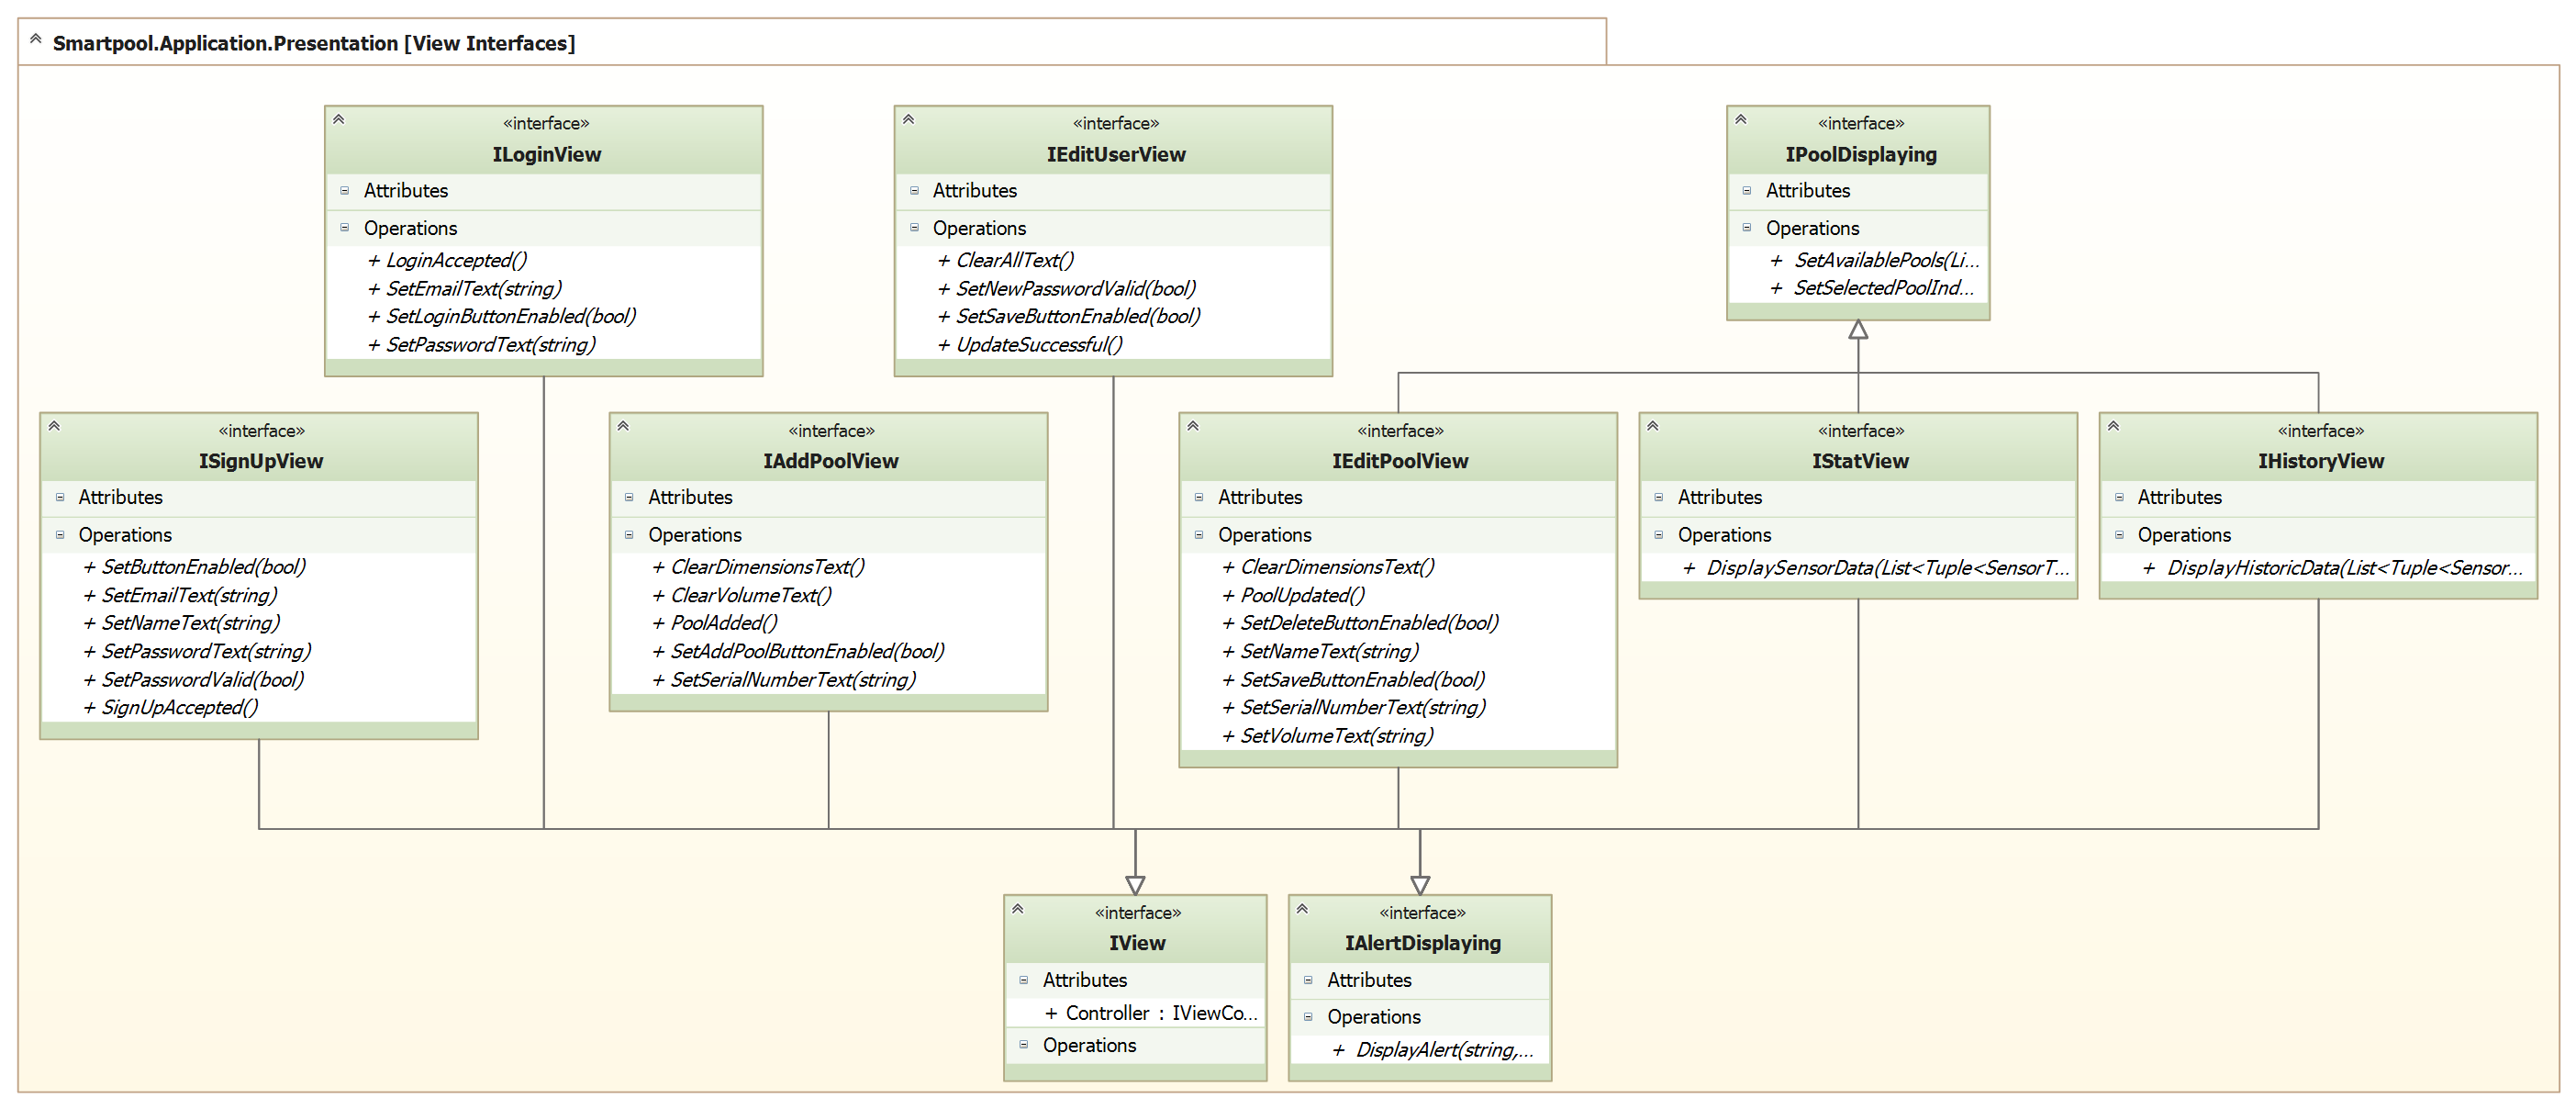
\includegraphics[width=1.0\linewidth]{figs/design/application_view_interfaces}
	\caption{View interfaces}
	\label{fig:application_view_interfaces}
\end{figure}

I de efterfølgende afsnit beskrives designet af applikationslagets view-interfaces.

\paragraph{IView}
Dette interface er det mest generelle view-interface, som implementeres af alle de andre views. Interfacet indeholder en property, Controller, som er en IViewController beskrevet i foregående afsnit. Alle views har derfor en controller, som de kan kalde ViewDidLoad på, eller typecaste til en mere specifik controller, som passer til det konkrete view.

\begin{figure}
	\centering
	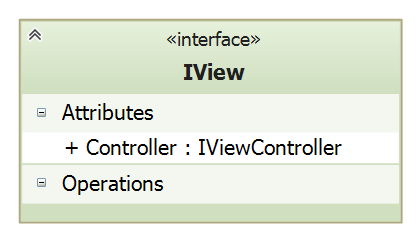
\includegraphics[width=0.3\linewidth]{figs/design/application_iview}
	\caption{IView}
	\label{fig:application_iview}
\end{figure}

\paragraph{IPoolDisplaying}
IPoolDisplaying er et andet generelt interface, som implementeres af alle de andre view-interfaces der har med visning af pool-oplysninger at gøre. Dette interface er segregeret fra de øvrige view-interfaces i forbindelse med projektets udvikling, da flere user stories, og dermed view-designs, indeholdte metoder til visning af pool-oplysninger. Interfacet indeholder metoder, som presenteren kan kalde, for at indlæse pool-oplysninger i view?et.

\begin{figure}
	\centering
	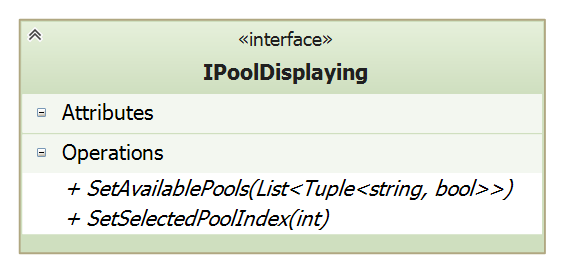
\includegraphics[width=0.4\linewidth]{figs/design/application_ipooldisplaying}
	\caption{IPoolDisplaying}
	\label{fig:application_ipooldisplaying}
\end{figure}

\paragraph{IAlertDisplaying}
IAlertDisplaying er det sidste generelle view-interface der er designet i dette lag. Det implementeres af alle de mere specifikke view-interfaces, der bør have mulighed for at vise en notifikation for brugeren.

\begin{figure}
	\centering
	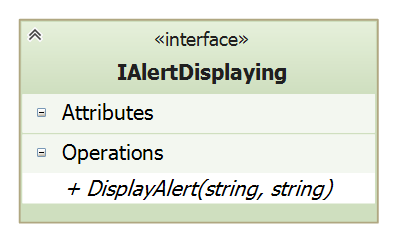
\includegraphics[width=0.3\linewidth]{figs/design/application_ialertdisplaying}
	\caption{IAlertDisplaying}
	\label{fig:application_ialertdisplaying}
\end{figure}

\paragraph{ISignUpView}
Dette interface er modparten til ISignUpViewController interfacet. ISignUpView indeholder dermed metoder til at opdatere view?ets tilstand, i form af tekstfelter og statusnotifikationer.

\begin{table}
	\centering
	\begin{tabular}{| l | p{0.7\linewidth} |}
		\toprule
		\textbf{Klassemedlem}	& \textbf{Beskrivelse} \\
		\midrule
		+ SetButtonEnabled(...)				& En metode der ændre på hvorvidt brugeren har mulighed for at gennemføre brugeroprettelse.	\\\hline
		+ SetEmailText(...)				& Metoder til at sætte teksten i view?ets tekstfelter. \\
		+ SetNameText(...)				& \\
		+ SetPasswordText(...)				& \\\hline
		+ SetPasswordValid(...) 					& En metode der notificerer view?et, om hvorvidt de indtastede passwords kan godkendes af systemet. \\\hline
		+ SignUpAccepted()				& En metode der notificerer view?et, om at brugeroprettelsen er gennemført af systemet. \\
		\bottomrule
		\end{tabular}
	\caption{Beskrivelse af ISignUpView-klassens medlemmer}
	\label{tab:table_design_isignupview}	
\end{table}

\paragraph{ILoginView}
ILoginView er modparten til ILoginViewController interfacet. Dette interface indeholder metoder som presenteren kan kalde, for at opdatere view?et under loginforsøg. Dette interface omhandler dermed, den user story, hvor en bruger ønsker at kunne logge ind i systemet.

\begin{table}
	\centering
	\begin{tabular}{| l | p{0.63\linewidth} |}
		\toprule
		\textbf{Klassemedlem}	& \textbf{Beskrivelse} \\
		\midrule
		+ LoginAccepted()				& En metode der notificerer view?et, når et login er gennemført.
	\\\hline
		+ SetEmailText(...)				& Metoder der sætter teksten i view?ets tekstfelter. \\
		+ SetPasswordText(...)				& \\\hline
		+ SetLoginButtonEnabled(...) 					& En metode der ændre på hvorvidt brugeren har mulighed for at gennemføre logge ind. \\
		\bottomrule
		\end{tabular}
	\caption{Beskrivelse af ILoginView-klassens medlemmer}
	\label{tab:table_design_iloginview}	
\end{table}

\paragraph{IAddPoolView}
Dette interface er modparten til IAddPoolViewController. Det indeholder metoder der tilgodeser de user stories, hvor en pool ønskes oprettet i systemet.

\begin{table}
	\centering
	\begin{tabular}{| l | p{0.6\linewidth} |}
		\toprule
		\textbf{Klassemedlem}	& \textbf{Beskrivelse} \\
		\midrule
		+ ClearDimensionsText()				& Metoder til at slette alt tekst i de pågældende tekstfelter. \\
		+ ClearVolumeText()					& \\\hline
		+ PoolAdded()				& En metode der kaldes af presenteren, når en pool er blevet tilføjet i systemet. \\\hline
		+ SetAddPoolButtonEnabled(...)				& En metode der ændre på hvorvidt brugeren har mulighed for at tilføje en pool. \\\hline
		+ SetSerialNumberText(...) 					& En metoder der sætter teksten i view?ets serienummer tekstfelt. \\
		\bottomrule
		\end{tabular}
	\caption{Beskrivelse af IAddPoolView-klassens medlemmer}
	\label{tab:table_design_iaddpoolview}	
\end{table}

\paragraph{IEditUserView}
IEditUserView interfacet indeholder metoder der kan kaldes af en IEditUserViewController, under redigering af pool-oplysninger.

\begin{table}
	\centering
	\begin{tabular}{| l | p{0.65\linewidth} |}
		\toprule
		\textbf{Klassemedlem}	& \textbf{Beskrivelse} \\
		\midrule
		+ ClearAllText()				& En metode der sletter alt tekst i view?ets tekstfelter. \\\hline
		+ SetPasswordValid(...)					& En metode der kan kaldes af presenteren, for at notificere view?et om hvorvidt de indtastede passwords kan godkendes.  \\\hline
		+ SetSaveButtonEnabled(...)				& En metode der ændre på hvorvidt brugeren har mulighed for at gemme ændringer om en pool.  \\\hline
		+ UpdateSuccessful()				& En metode der kaldes når en pool opdatering er gennemført af systemet. \\
		\bottomrule
		\end{tabular}
	\caption{Beskrivelse af IEditUserView-klassens medlemmer}
	\label{tab:table_design_iedituserview}	
\end{table}

\paragraph{IEditPoolView}
Dette interface er modparten til IEditPoolViewController, og omhandler dermed redigering af pool-oplysninger. Interfacet indeholder en række metoder til at sætte tilstanden i de tekstfelter og knapper der vurderes nødvendige i views af denne type.

\begin{table}
	\centering
	\begin{tabular}{| l | p{0.62\linewidth} |}
		\toprule
		\textbf{Klassemedlem}	& \textbf{Beskrivelse} \\
		\midrule
		+ ClearDimensionsText()				 &En metode der sletter alt tekst om poolens størrelse. \\\hline
		+ PoolUpdated()					& En metode der kaldes når en pool er blevet opdateret i systemet. \\\hline
		+ SetDeleteButtonEnabled(...)				& Metoder der kaldes, for at ændre på tilstanden af knapperne i view?et. \\
		+ SetSaveButtonEnabled(...)				& \\\hline
		+ SetNameText(...)						& Metoder der kaldes, for at sætte teksten i view?ets tekstfelter.
 \\
		+ SetSerialNumberText(...)				& \\
		+ SetVolumeText(...)						& \\
		\bottomrule
		\end{tabular}
	\caption{Beskrivelse af IEditPoolView-klassens medlemmer}
	\label{tab:table_design_ieditPoolview}	
\end{table}

\paragraph{IStatView}
IStatView er modparten til IStatViewController. Dette interface indeholder en metode, der skal kunne indlæse sensor data i view?et. Sensor data bliver sendt som en liste af tupler, med sensor type og måleværdi.

\begin{figure}
	\centering
	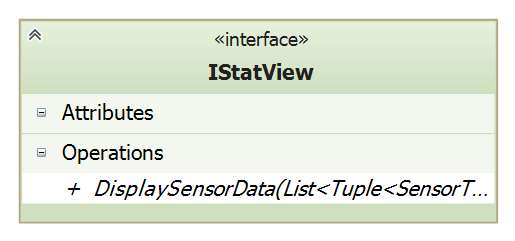
\includegraphics[width=0.3\linewidth]{figs/design/application_istatview}
	\caption{IStatView}
	\label{fig:application_istatview}
\end{figure}

\paragraph{IHistoryView}
Dette interface er modparten til IHistoryViewController. Interface indeholder en metode, der skal kunne indlæse historisk sensor data i view?et. Sensor data bliver sendt som en liste af tupler, med sensor type og en liste af måleværdier.

\begin{figure}
	\centering
	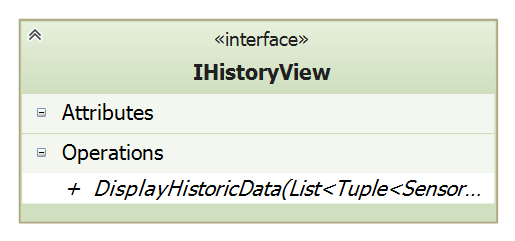
\includegraphics[width=0.3\linewidth]{figs/design/application_ihistoryview}
	\caption{IHistoryView}
	\label{fig:application_ihistoryview}
\end{figure}

\subsubsection{Presenter-klasser}
Efter at have designet par af view- og presenter-interfaces, blev konkrete presenter-klasser designet. De implementerer et presenter-interface, samt indeholder det view-inteface, som presenteren bør kobles sammen med.

Presenter-klasserne er designet til at være platform-uafhængige, ved ikke at benytte klasser, som ikke understøttes i portable projekter. Da klasserne er designet sammen med interfaces, giver det stadigvæk mulighed for, at lave specifikke presenters for en given platform, hvis det bliver nødvendigt. Alle presenters har en constructor, der tager imod en IClientMessenger (defineret i connection-modellen), og et view af den tilhørende type. Presenter-klasserne har brug for at modtage en IClientMessenger fra view?et der instantiere presenteren, for at platform specifikke klienter ikke skal forhindre præsentationslaget i at være portabelt. 

\begin{landscape}
\begin{figure}
	\centering
	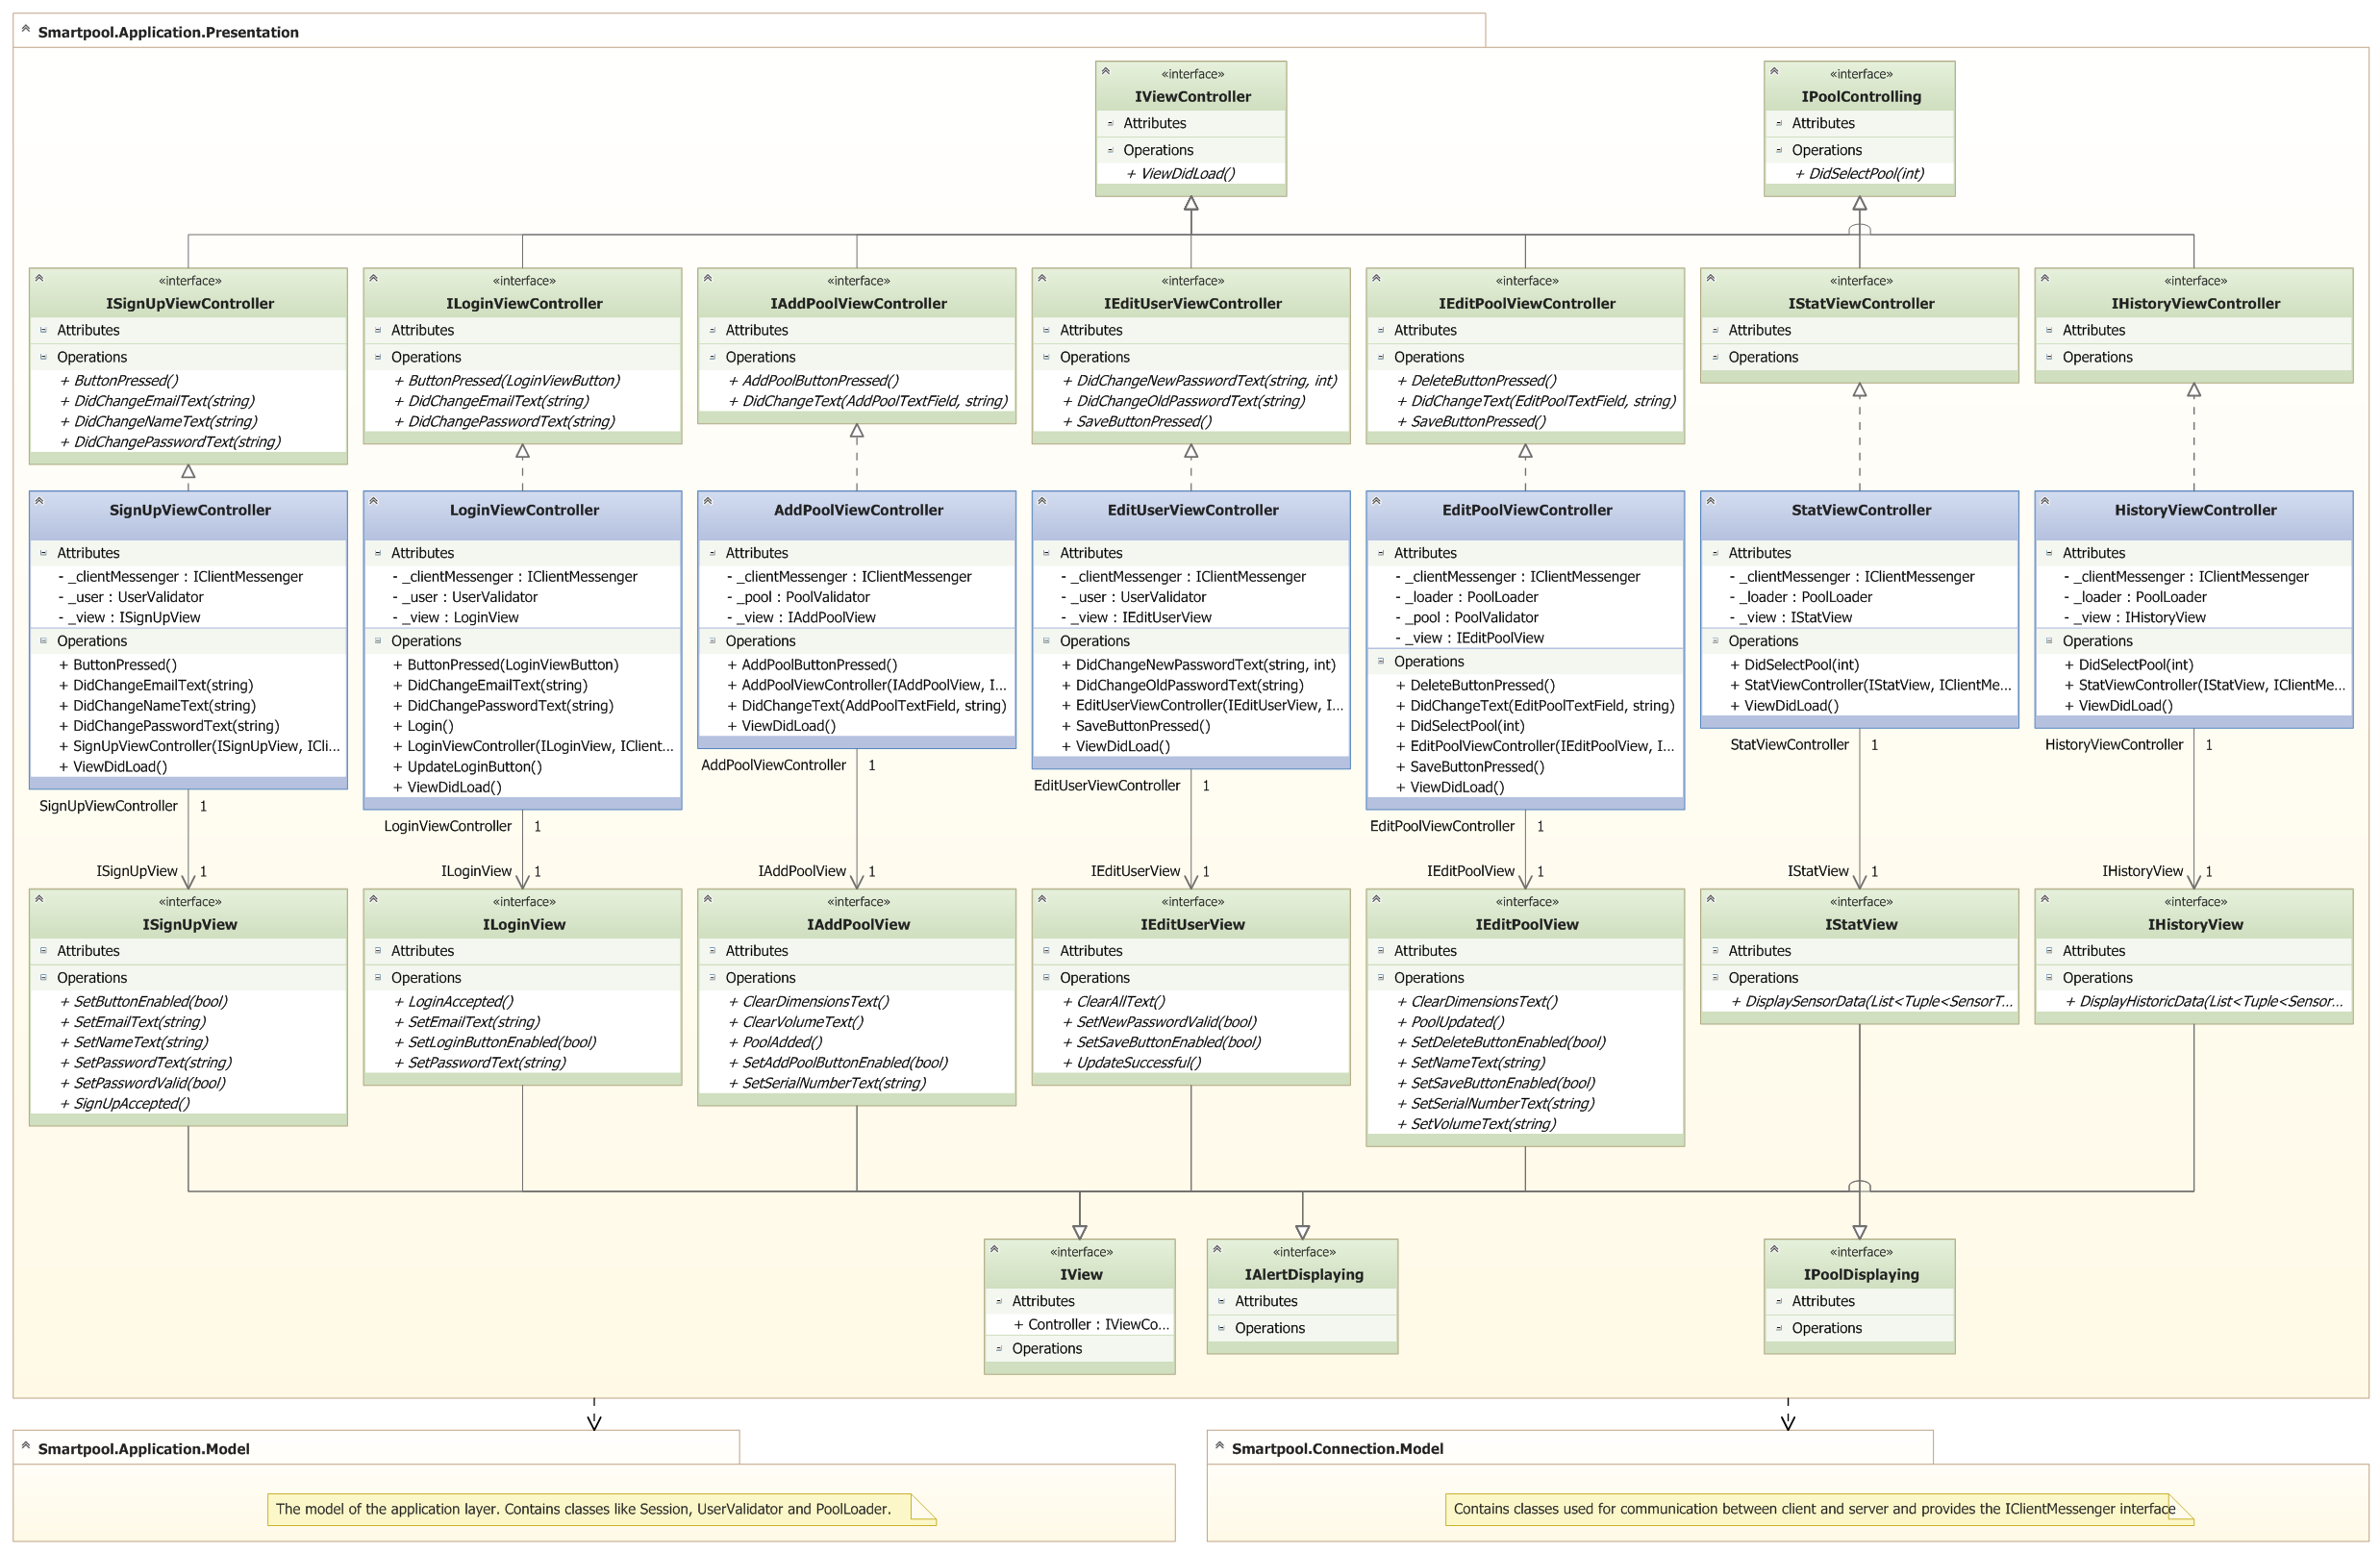
\includegraphics[width=1\linewidth]{figs/design/application_presentation_full}
	\caption{Klasser og interfaces i præsentationslaget}
	\label{fig:application_presentation_full}
\end{figure}
\end{landscape}

I de efterfølgende afsnit beskrives kort, de metoder og properties, der er tilføjet designet af de konkrete presenters, og som ikke er beskrevet ved deres interface.

\paragraph{SignUpViewController}
SignUpViewController-klassen implementerer ISignUpViewController interfacet. Klassen indeholder en række private felter, til at gemme en reference til de parametre der medsendes i constructoren. Derudover indeholder klassen en UserValidator fra modellaget, da denne type presenter har brug for en metode til, at verificere oplysninger ved brugeroprettelse.

\begin{figure}
	\centering
	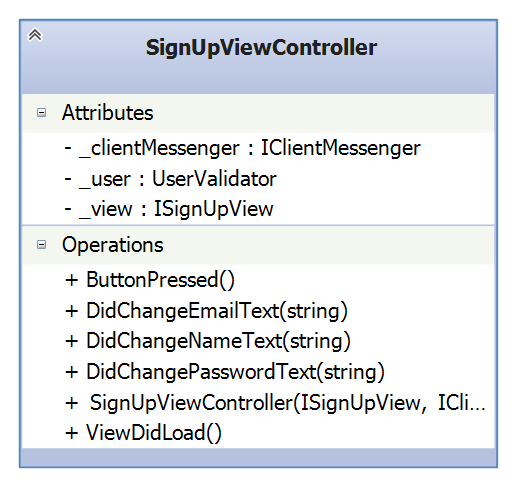
\includegraphics[width=0.3\linewidth]{figs/design/application_signupviewcontroller}
	\caption{SignUpViewController}
	\label{fig:application_signupviewcontroller}
\end{figure}

\paragraph{LoginViewController}
LoginViewController-klassen implementerer ILoginViewController interfacet. Klassen indeholder en række private felter, til at gemme en reference til de parametre der medsendes i constructoren. Derudover indeholder klassen en UserValidator, som presenteren kan benytte til verificering af loginoplysninger.

\begin{figure}
	\centering
	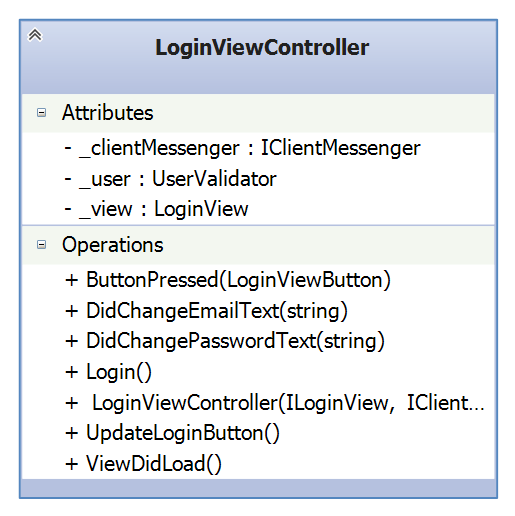
\includegraphics[width=0.3\linewidth]{figs/design/application_loginviewcontroller}
	\caption{LoginViewController}
	\label{fig:application_loginviewcontroller}
\end{figure}

\paragraph{AddPoolViewController}
AddPoolViewController-klassen implementerer IAddPoolViewController interfacet. Klassen indeholder en række private felter, til at gemme en reference til de parametre der medsendes i constructoren. Da denne type presenter ifølge interfacet håndterer tilføjelse af nye pools, indeholder klassen også en PoolValidator fra modellaget, til validering af brugerens input.

\begin{figure}
	\centering
	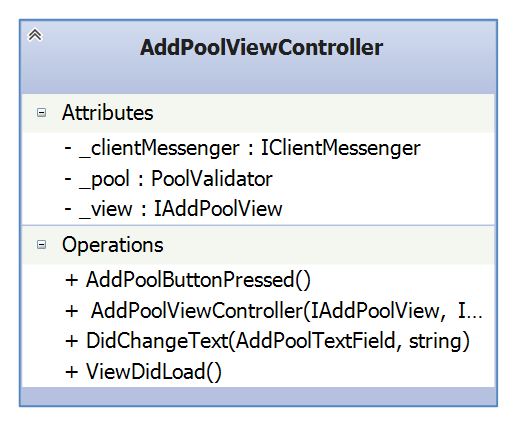
\includegraphics[width=0.3\linewidth]{figs/design/application_addpoolviewcontroller}
	\caption{AddPoolViewController}
	\label{fig:application_addpoolviewcontroller}
\end{figure}

\paragraph{EditUserViewController}
EditUserViewController-klassen implementerer IEditUserViewController interfacet. Klassen indeholder en række private felter, til at gemme en reference til de parametre der medsendes i constructoren. Klassen har også en UserValidator til verificeing af brugeroplysninger.

\begin{figure}
	\centering
	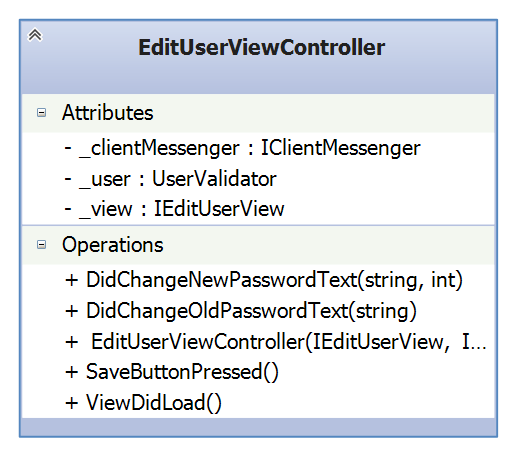
\includegraphics[width=0.3\linewidth]{figs/design/application_edituserviewcontroller}
	\caption{EditUserViewController}
	\label{fig:application_edituserviewcontroller}
\end{figure}

\paragraph{EditPoolViewController}
Denne klasse implementerer IEditPoolViewController interfacet. Ud over de parametre der medsendes i constructoren, indeholder klassen en PoolValidator fra modellaget, samt en PoolLoader. PoolLoaderen er nødvendig for presenterens design, da den skal løse opgaver omhandlende indhentning af pool-oplysninger.

\begin{figure}
	\centering
	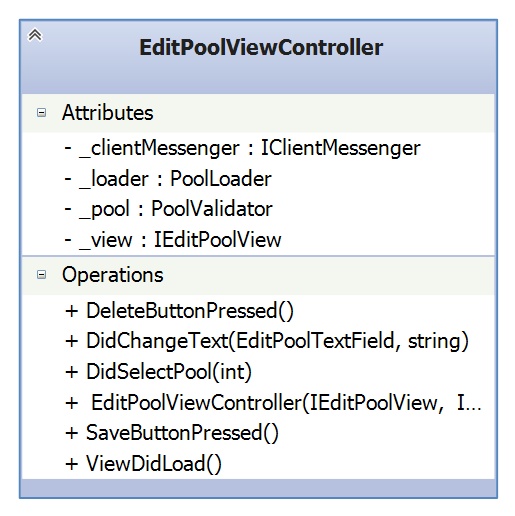
\includegraphics[width=0.3\linewidth]{figs/design/application_editpoolviewcontroller}
	\caption{EditPoolViewController}
	\label{fig:application_editpoolviewcontroller}
\end{figure}

\paragraph{StatViewController og HistoryViewController}
StatViewController og HistoryViewController implementerer hhv. IStatViewController og IHistoryViewController interfacene. Begge presenter-klasser indeholder private felter til at gemme de parametre der modtages i constructoren, samt en PoolLoader, da begge klasser skal kunne indlæse pool-oplysninger.

\begin{figure}
	\centering
	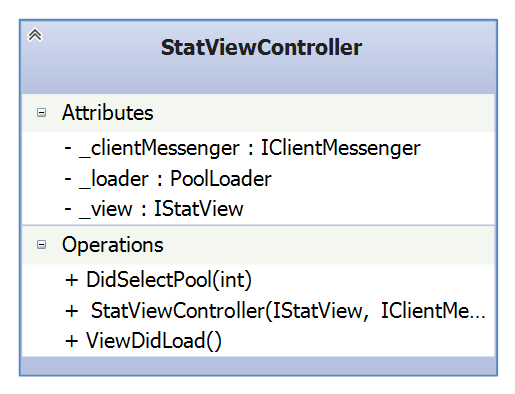
\includegraphics[width=0.3\linewidth]{figs/design/application_statviewcontroller}
	\caption{StatViewController}
	\label{fig:application_statviewcontroller}
\end{figure}